
% JuliaCon proceedings template
\documentclass{juliacon}
\setcounter{page}{1}
\usepackage{verbatim}
\usepackage{amsmath}

\begin{document}

% **************GENERATED FILE, DO NOT EDIT**************

\title{GeometricFlux.jl: a geometric deep learning library in Julia}

\author[1, 2]{Yueh-Hua Tu}
\affil[1]{Bioinformatics Program, Taiwan International Graduate Program, Institute of Information Science, Academia Sinica, Taipei, 11529, Taiwan}
\affil[2]{Graduate Institute of Biomedical Electronics and Bioinformatics, National Taiwan University, Taipei, 10617, Taiwan}

\keywords{Julia, Geometric deep learning, Graph neural network, Machine learning, Geep learning}

\hypersetup{
pdftitle = {GeometricFlux.jl: a geometric deep learning library in Julia},
pdfsubject = {JuliaCon 2019 Proceedings},
pdfauthor = {Yueh-Hua Tu},
pdfkeywords = {Julia, Geometric deep learning, Graph neural network, Machine learning, Geep learning},
}



\maketitle

\begin{abstract}

Data from various fields have their suitable structure. Nowadays, applicable data in
artificial intelligence are images, text and speech. These data can be represented as vector
or matrix structure. However, some data are not suitable for matrix structure or it can be
sparse to fit in matrix structure. For example, social network in social science, biological
network in biology and traffic network represent their data in graph or network structure.
Usually, measurement of these data lies in non-Euclidean space. To utilize network
representation as input for deep learning model, geometric deep learning, or its subfield
called graph neural network, learns topological information provided by network structure
and latent information from input features simultaneously. A geometric deep learning
framework in Julia is proposed, GeometricFlux.jl. GeometricFlux.jl is a Julia package for
geometric deep learning on graph. It extends Flux.jl, a well-known machine learning
framework in Julia, to accept network structure as model input. Some well-known and key
graph convolutional layers are implemented in GeometricFlux.jl. It relies on Zygote.jl for
automatic differentiation engine. ScatterNNlib.jl acted as independent package contains
essential scatter/gather operations and their gradient for GeometricFlux.jl. To leverage
existing JuliaGraphs ecosystem, GeometricFlux.jl accepts graph data structure constructed
from JuliaGraphs. Layers implemented in GeometricFlux.jl are compatible with Flux.jl layers.
Thus, dropout, batch normalization and dense layers are applicable when using Flux and
GeometricFlux.jl together. GPU computation is necessary and is supported by CUDA.jl as well.
Static and variable graphs are supported for efficiency and various network structure input,
respectively. Message-passing scheme \cite{gilmer2017} and graph network block \cite{battaglia2018}
are implemented as flexible and integrated framework. The performance of scatter operations
are benchmarked and it outperforms pytorch-scatter on cuda. I propose a novel and competitive
geometric deep learning library in Julia.

\end{abstract}

\section{Introduction}

Geometric deep learning emerges as a subfield of deep learning. It learns with irregular
structured data and features. Topological information from graph is embedded with features
through the whole neural network. Graph neural network provides a generic approach [@Gilmer:2017; @Battaglia:2018]
for learning topological information together with features to get precisely prediction.
However, integration of scientific computing, software architecture, graph representation
and dataset preparation is challenging. GPU computation on irregular data struture is not
commonly supported. A well-defined graph neural network framework is needed for researchers
to operate with. I proposed GeometricFlux, a geometric deep learning extension of a deep learning
library, Flux, in Julia. Graph convolutional layers are organized in the design of message
passing scheme. Graph network block is implemented as a generic version of message passing
scheme. Leveraging Julia ecosystem, operations on CPU and GPU are optimized with SIMD and
CUDA.jl, respectively. Graph representations are supported with general array or graphs from
JuliaGraph ecosystem.
A github repository is available in https://github.com/yuehhua/GeometricFlux.jl.

\begin{figure*}[t]
\centerline{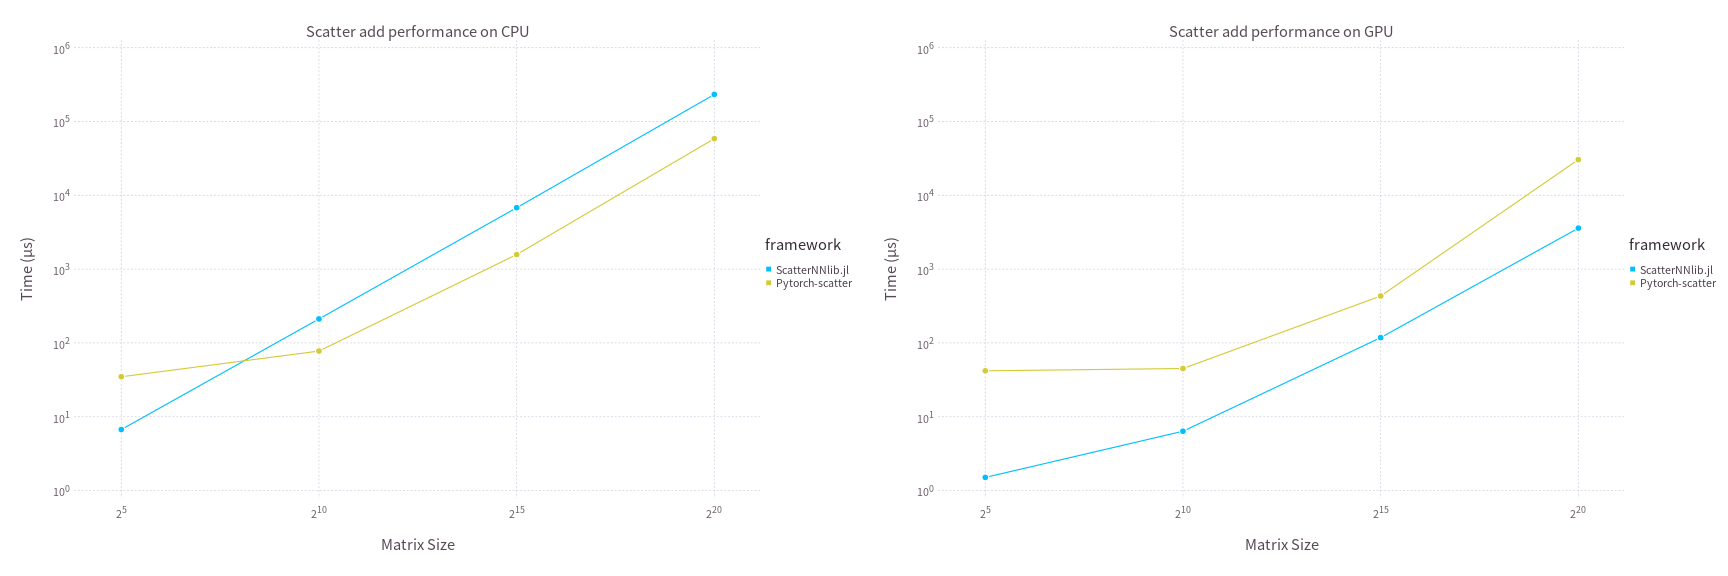
\includegraphics[width=18cm]{figures/scatter_add.svg}}
\caption{Benchmark for scatter add on CPU and GPU.}
    \label{fig:scatter_add}
\end{figure*}

\begin{figure*}[h]
\centerline{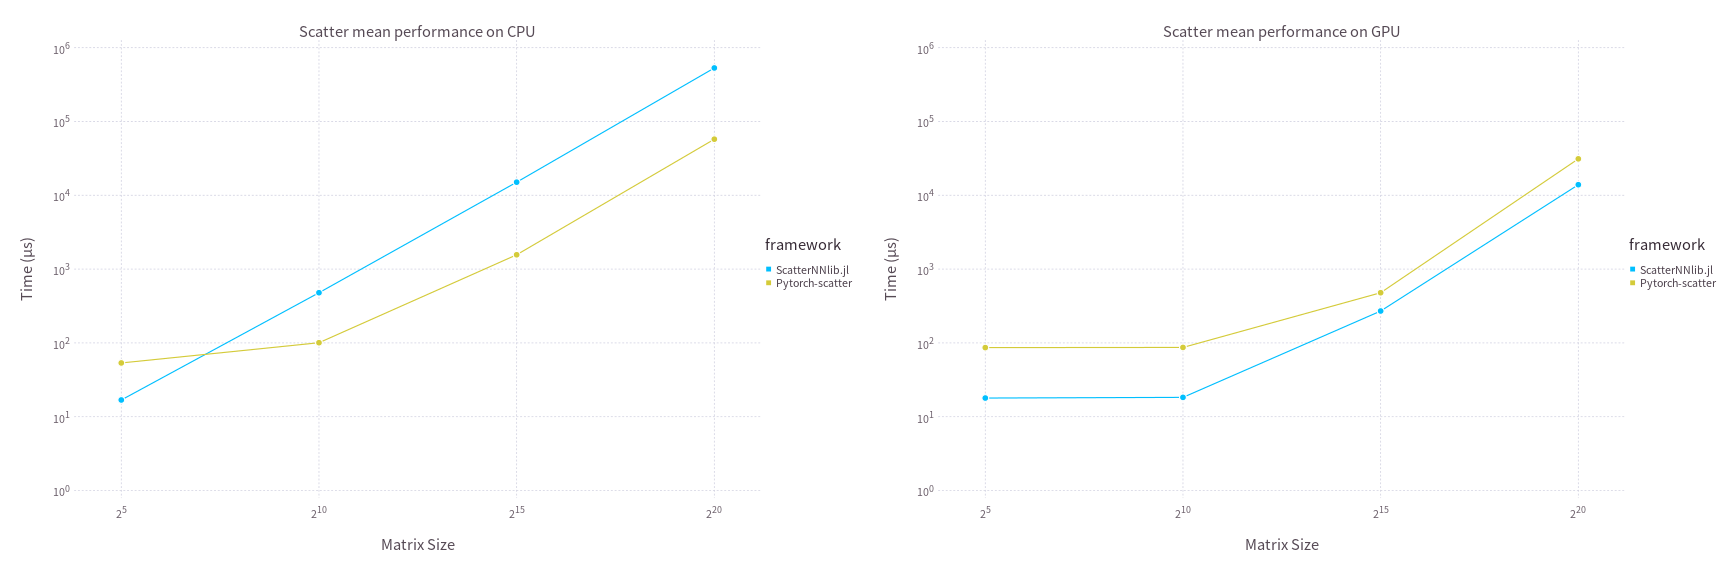
\includegraphics[width=18cm]{figures/scatter_mean.svg}}
\caption{Benchmark for scatter mean on CPU and GPU.}
    \label{fig:scatter_mean}
\end{figure*}

\begin{figure*}[h]
\centerline{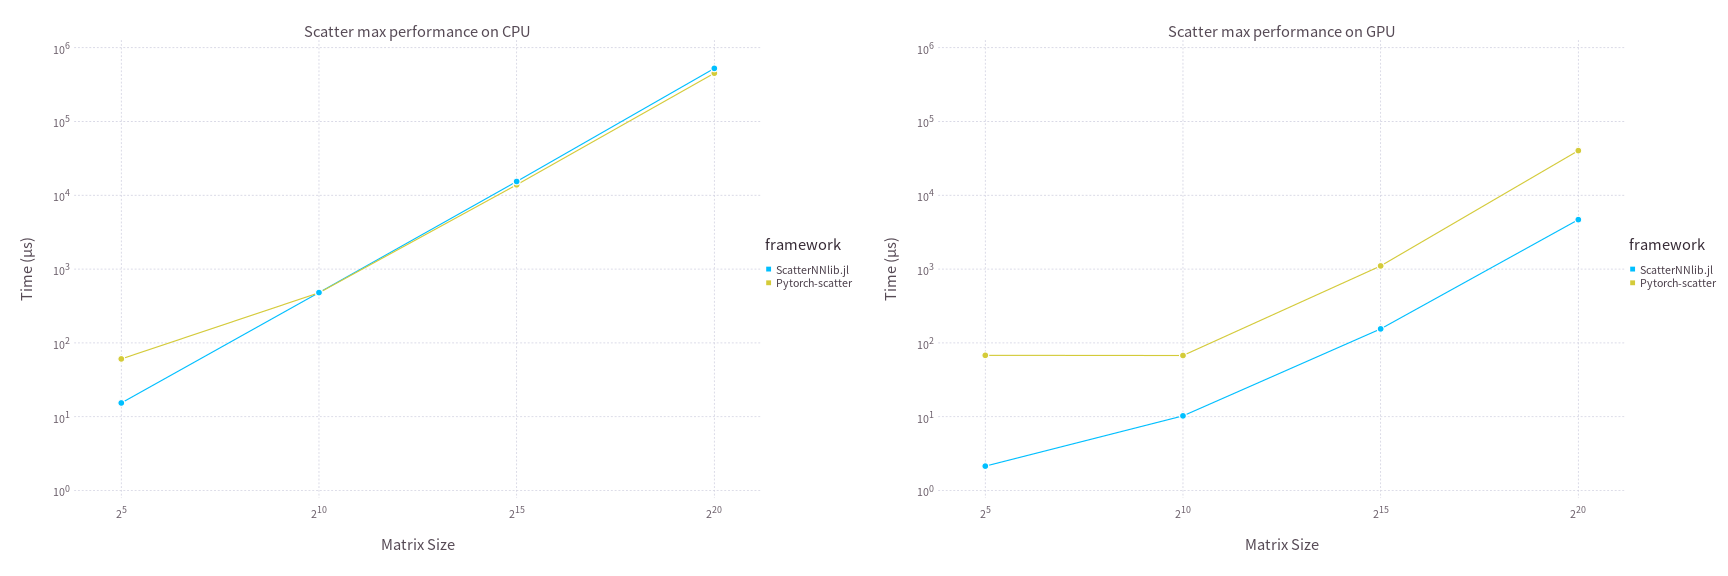
\includegraphics[width=18cm]{figures/scatter_max.svg}}
\caption{Benchmark for scatter max on CPU and GPU.}
    \label{fig:scatter_max}
\end{figure*}

\section{Extending Framework}

An extending framework is designed to integrate message-passing scheme and graph network (GN)
block in GeometricFlux. Message-passing scheme is defined in two functions: message function
and update function. Message function passes states on node itself and its neighbors or edges
and give messages. Aggregate function is used to aggregate messages into single outcome.
Update function takes node state and aggregated message, and then update the result as new
node state. Precisely, message-passing scheme can be described as follow:

\[
    \begin{aligned}
    m_i^{(t+1)} &= agg_{j \in \mathcal{N}(i)}(M(x_i^{(t)}, x_j^{(t)}, e_{ij})) \\
    x_i^{(t+1)} &= U(x_i^{(t)}, m_i^{(t+1)})
    \end{aligned}
\]

Message function $M$ and update function $U$ are predefined by a network layer or users.
A message for node $i$ is calculated for $t+1$-th layer, which is denoted as $m_i^{(t+1)}$,
and aggregated in elementwise manner by operation $agg$ with neighbors of $i$. A new node $i$
state $x_i^{(t+1)}$ is computed for $t+1$-th layer as an outcome from update function.

GN block defines a more general operations on graph. It updates edge, node and global states
individually. Aggregate functions are applied after updating states and merge states from edges
to nodes, from edges to global and from nodes to global. GN is implemented as an abstract
type in Julia and coupled with a series of update functions and aggregate functions as API
for overriding. As a special case of GN, message-passing network is defined as subtype of GN.
Update functions are defined as follow:

\[
    \begin{aligned}
    e_k' &= \phi^e (e_k, v_i, v_j, g) \\
    v_i' &= \phi^v (\bar{e}_i', v_i, g) \\
    g' &= \phi^g (\bar{e}', \bar{v}', g)
    \end{aligned}
\]

and aggregate functions are

\[
    \begin{aligned}
    \bar{e}_i' &= \rho^{e \rightarrow v} (\{e_k', i, j\}_{j \in \mathcal{N}(i),k = (i, j)}) \\
    \bar{e}' &= \rho^{e \rightarrow g} (\{e_k\}_{k \in E}) \\
    \bar{v}' &= \rho^{v \rightarrow g} (\{v_i\}_{i \in V})
    \end{aligned}
\].

New states for edges, nodes and global graph are updated by $\phi^e$, $\phi^v$ and $\phi^g$,
respectively. $\phi^e$ takes edge state $e_k$, corresponding node state $v_i$, $v_j$ and
global state $g$, and then outputs a new edge state $e_k'$ for edge $k$.
$\rho^{e \rightarrow v}$ aggregates states of edge incident to node $i$.
$\rho^{e \rightarrow g}$ and $\rho^{v \rightarrow g}$ functions aggregate all edge states and
node states into a global state, respectively. It is designed as a whole in single layer
such that a GN block can be use as an unit of a neural network.

\section{Static and Variable Graph Support}

In graph neural network, static graph structure is required for computation efficiency;
while variable graph carried by input features is used to train neural network on various
graph topology. Static graph should be given during constructing GNN layers; while variable
graph is packed within FeaturedGraph data structure as input of GNN layer. Static graphs are
processed for efficiency in prior during constructing GNN layer and variable graphs are
processed during network training time. In this framework, graph network block is designed as
fundamental layers. Each layer accepts input of node features, edge features, global features
and graph. Graph structures from LightGraphs.jl, SimpleWeightedGraphs.jl and MetaGraphs.jl
are accepted. FeaturedGraph is designed as generic data structure for containing different
kinds of features and graph structure.

\section{Compatible with Flux Layers}

In general, the layer design of graph neural network is different from regular layer of
neural network. The layer of graph neural network accepts at least features and graph as input.
In our architecture, we accept node features, edge features, global features and graph as input.
To make layer design compatible with regular neural network needs complicated design in
each GNN layer. GNN layers are designed with two version, one for FeaturedGraph input and
the other for normal feature input. GNN layers are designed to be consistent with input type
and output type. Output of regular feature will be the input of regular Flux layer.
Conclusively, layers implemented in GeometricFlux are compatible with regular Flux layers.

\section{Integration with JuliaGraphs}

JuliaGraphs already forms a whole ecosystem for graph operations, graph visualization and
solving problems in graph theory. LightGraphs.jl and SimpleWeightedGraphs.jl provides the
graph construction and representation in unweighted and weighted graphs.
MetaGraphs.jl provides user the chance to assign properties on nodes, edges or global graph.
Integration with JuliaGraphs ecosystem provides more ways to assign graph to model and
reduce the effort of transformation between data types. Graph representation constructed
from LightGraphs.jl, SimpleWeightedGraphs.jl and MetaGraphs.jl are accepted in construction
of geometric deep learning model in GeometricFlux. Under construction of graph convolutional
layer, a static graph is accepted as one of arguments of neural network layer during
configuring model. In the context of using variable graph, FeaturedGraph also accepts graph
representation constructed from LightGraphs.jl, SimpleWeightedGraphs.jl and MetaGraphs.jl
and can be fed as sample directly to model. This feature accepts graph representations
from JuliaGraphs ecosystem to geometric deep learning model.

\section{Performance Evaluation}

Julia community is always interested to performance issues of all kinds of computation.
Scatter functions are benchmarked to show the fundamental operations in graph neural network
model. Matrix addition and multiplication is to convolutional neural network as scatter
operations is to graph neural network. I compared time consumption on scatter add function
between pytorch geometric and GeometricFlux. The functionality of scatter operations are
separated as independent packages of pytorch scatter and ScatterNNlib for pytorch geometric
and GeometricFlux, respectively. Benchmark are performed on Intel i7-8700K machine with a
Nvidia Titan XP and Ubuntu 20.04 64-bit. Software of ScatterNNlib.jl v0.1.1 and CUDA.jl v1.2.1
with Cuda version of 10.1 is used. For pytorch, Pytorch v 1.6.0 and Pytorch-scatter v 2.0.5
are tested. I benchmarked on both CPU and GPU with scatter add (\autoref{fig:scatter_add}), mean (\autoref{fig:scatter_mean})
and max (\autoref{fig:scatter_max}).

\section{Datasets Preparation}

Datasets are preprocessed and prepared by GraphMLDatasets.jl. Currently, the citation graphs
Cora, CiteSeer, PubMed and Cora-Full datasets \cite{sen2008,bojchevski2018deep} are
provided. Scientific datasets such as molecule datasets QM7b \cite{montavon2013} and
protein-protein interaction graphs \cite{hamilton2017} are also provided.

\section{Conclusion}

I introduced GeometricFlux for deep learning on graph. An extending framework is designed
to be the core of GeometricFlux and it also supports of static and variable graph.
JuliaGraph ecosystem is also integrated to provide more graph representations.
Effective scatter operations are implemented to accelerate model training and inference.
These make GeometricFlux as a prototype of playground for geometric deep learning in Julia.
Finally, I will keep working to implement more network layers on graph and more prepared
datasets.

\section{Acknowledgments}

I personally thank Ching-Wen Cheng for suggestions on scatter operation implementation.

% **************GENERATED FILE, DO NOT EDIT**************

\bibliographystyle{juliacon}
\bibliography{paper.bib}


\end{document}

% Inspired by the International Journal of Computer Applications template
